\documentclass[a4paper,12pt]{article}
\usepackage[english]{babel}
\usepackage[utf8]{inputenc}
\usepackage{setspace}

% Larger borders -- we do not want do waste paper, even if it is only paper on screen =)
\usepackage[top=2.5cm, bottom=2.5cm, left=2cm, right=2cm]{geometry}
% Remove auto indentation of paragraphs.
\setlength\parindent{0pt}

% Palatino font (nicer serif font: Times is for oldies)
%\renewcommand*\rmdefault{ppl}

% Nested itemize list bullet style
\renewcommand{\labelitemi}{$\bullet$}
\renewcommand{\labelitemii}{$\circ$}
\renewcommand{\labelitemiii}{--}

% Math packages
\usepackage{mathtools}
\usepackage{amsmath}
\usepackage{amsfonts}
\usepackage{amssymb}

% Graphic packages
\usepackage{graphicx}
\usepackage{float}
\usepackage{adjustbox}
\usepackage{tikz}
\usepackage{forest,array}
\usetikzlibrary{shadows}

% Graphs styles
\forestset{
  giombatree/.style={
    for tree={
      grow = east,
      parent anchor=east,
      child anchor=west,
      edge={rounded corners=2mm},
      fill=violet!5,
      drop shadow,
      l sep=10mm,
      edge path={
        \noexpand\path [draw, \forestoption{edge}] (!u.parent anchor) -- +(5mm,0) -- (.child anchor)\forestoption{edge label};
      }
    }
  }
}
\forestset{
  qtree/.style={
    for tree={
      parent anchor=south,
      child anchor=north,
      align=center,
      edge={rounded corners=2mm},
      fill=violet!5,
      drop shadow,
      l sep=10mm,
    }
  }
}

% BAN logic macros
\newcommand{\believes}{\mid\!\equiv}
\newcommand{\sees}{\triangleleft}
\newcommand{\oncesaid}{\mid\!\sim}
\newcommand{\controls}{\Rightarrow}
\newcommand{\fresh}[1]{\#(#1)}
\newcommand{\combine}[2]{{\langle #1 \rangle}_{#2}}
\newcommand{\encrypt}[2]{{ \{ #1 \} }_{#2}}
\newcommand{\sharekey}[1]{\xleftrightarrow{#1}}
\newcommand{\pubkey}[1]{\xmapsto{#1}}
\newcommand{\secret}[1]{\xleftrightharpoons{#1}}

\newcommand{\projectname}{Aeronautical Communication System}
\newcommand{\projectnameabbr}{ACS}

% Hides ugly links from the index
\usepackage[hidelinks]{hyperref}
% Landscape format pdf pagess
\usepackage{pdflscape}


\begin{document}
\pagenumbering{gobble}

{\setstretch{1.0}
  \begin{titlepage}
  	\centering
  	
\includegraphics[width=6cm]{img/unipi.pdf}\par
    \vspace{1.5cm}
    {\Large Department of Information Engineering \par}
  	\vspace{1.5cm}
  	{\huge\textsc{\projectname{}}\par}
    \vspace{0.5cm}
    {\Large Performance Evaluation of Computer Systems and Networks project \par}
  	\vspace{2cm}
  	Pietro \textsc{Gronchi}\par
  	Amedeo \textsc{Pochiero}\par
    Giovan Battista \textsc{Rolandi}

  	\vfill

    % Bottom of the page
  	{\large A.Y. 2019-2020\par}
  \end{titlepage}
}


\clearpage
~
\clearpage
\tableofcontents
\clearpage
~
\clearpage
\pagenumbering{arabic}

\section{Introduction}
\projectname{} is a cummunication system between aircrafts (AC) and a control tower (CT).
Connection between AC and CT is provided by ground base stations (BS), which are deployed over a grid, at a distance M from neighbors.

\begin{figure}[H]
  \centering
  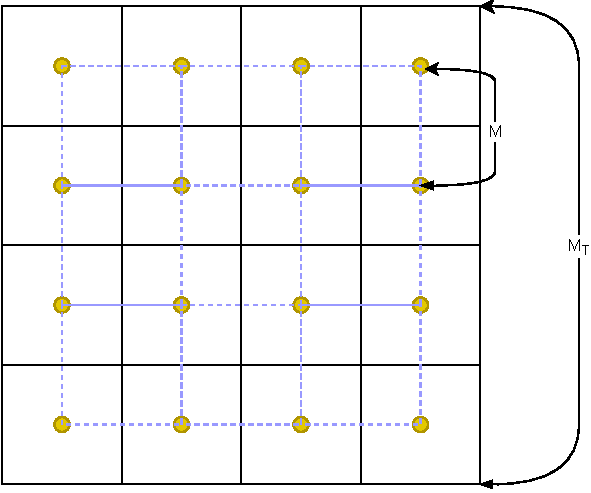
\includegraphics[width=6cm]{img/grid.pdf}
  \caption{System topology}
  \label{fig:grid}
\end{figure}

Deployment grid has a square topology, eg. number of rows is equal to number of columns.
In Figure~\ref{fig:grid}, deployment grid is drawn with dotted blue lines, while solid black lines delimit the area, called \emph{cell}, where an AC is closer to the inner base station.
$L$ is a shortcut to indicate $M \cdot n$, where $n$ is the number of BSs that lay on a row (or a column).

Each AC selects only one BS at a time as its serving BS, and can transmit only one packet at a time.
Possibly, packets are backlogged in a queue on the AC.

ACs execute the handover procedure every $t$ seconds, accordingly with the following algorithm:
\begin{verbatim}
if (serving BS is the closest one) then
  do nothing
else
  select closest BS as serving BS
  pause transmissions for penalty time (p)
endif
\end{verbatim}

\subsection{Constant and variables summary}
\begin{itemize}
  \item \textbf{k}: it represents the interarrival time of packets;
  \item \textbf{M}: it represents the distance between two consecutive BS on the same row, or column, and it is fixed at 25 km;
  \item \textbf{d}: it represents the distance between AC and BS;
  \item \textbf{s}: it represents the service time of a packet, and is given by $s = T \cdot d^{2}$;
  \item \textbf{T}: it is a tuning parameter for service time, whose value is costant for every AC in the system;
  \item \textbf{t}: it represents the handover period;
  \item \textbf{p}: it represents the handover penalty;
\end{itemize}

\section{Model}
% TODO high level model

Service time depends on distance between AC and BS.
Distance between AC and BS, namely \emph{d}, belongs to interval $[ 0, d_{max} [$ where $d_{max}$ can be computed as $d_{max\_in} + d_{max\_out}$, where:
\begin{itemize}
  \item $d_{max\_in} = \frac{M \sqrt{2}}{2} $
  \item $d_{max\_out} = vt$
\end{itemize}

\begin{figure}[H]
  \centering
  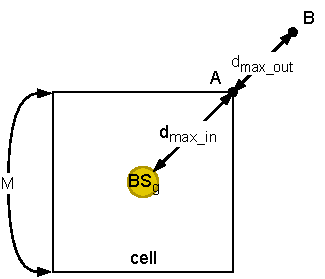
\includegraphics{img/dmax.pdf}
  \caption{Computation of $d_{max}$}
  \label{fig:dmax}
\end{figure}

What is the worst case? Referring to Figure~\ref{fig:dmax}, let's assume that an AC is moving in direction $BS_g \rightarrow B$, and that, at a given time $t_g$, $\overrightarrow{AC} \in cell$ and $\overrightarrow{AC} - \overrightarrow{A} < \epsilon$ with $\epsilon$ small as you wish, eg. AC is at point A but still inside the cell where the nearest BS is $BS_g$; and let's assume that, at this time, AC initiates the handover procedure and discovers that the nearest BS is $BS_g$. Immediately after this handover procedure, performed without any penalty time, AC is out of the cell and will not initiate the handover procedure before $t$ time: this means that, when it is in point B, it has traveled for, $d_{max\_out} = v t$, since the last handover procedure, and that the longest distance $d_{max}$ between AC and BS is given by:

$$ d_{max} = \frac{M \sqrt{2}}{2} + vt $$

\subsection{Movement of AC}
Movement of AC is given by the following algorithm, implemented using the \texttt{TurtleMobility} module from INET:
\begin{itemize}
  \item generate a vector $\vec{s}$ such that $|\vec{s}| \in \mathcal{U}(0, M_{T}\sqrt{2})$ and $\angle{s} \in \mathcal{U}(0, 2\pi)$; upper bound of $\vec{s}$ is maximum possibile distance before AC surely wraps around;
  \item given that AC is in position $\vec{a}$, move to position $\vec{a} + \vec{s}$, at constant $v$ speed, possibly wrapping around at the edges of the simulated topology;
  \item once reached new position, re-do from the beginning;
\end{itemize}


\end{document}
